% Created 2024-06-05 mié 23:44
% Intended LaTeX compiler: pdflatex
\documentclass[presentation]{beamer}
\usepackage[utf8]{inputenc}
\usepackage[T1]{fontenc}
\usepackage{graphicx}
\usepackage{grffile}
\usepackage{longtable}
\usepackage{wrapfig}
\usepackage{rotating}
\usepackage[normalem]{ulem}
\usepackage{amsmath}
\usepackage{textcomp}
\usepackage{amssymb}
\usepackage{capt-of}
\usepackage{hyperref}
\usetheme{Madrid}
\usecolortheme{}
\usefonttheme{}
\useinnertheme{}
\useoutertheme{}
\author{Luis Enrique Perez Señalin}
\date{\textit{<2024-06-05 mié>}}
\title{Deber elaboracion procesadores}

\hypersetup{
 pdfauthor={Luis Enrique Perez Señalin},
 pdftitle={Deber elaboracion procesadores},
 pdfkeywords={},
 pdfsubject={},
 pdfcreator={Emacs 27.1 (Org mode 9.3)}, 
 pdflang={Spanish}}
\begin{document}

\maketitle
\begin{frame}{Outline}
\tableofcontents
\end{frame}


\section{Procesos}
\label{sec:orgeafec88}
\begin{frame}[label={sec:org5436396}]{Presentacion0}
Pasos para la elaboración de un microprocesador
\end{frame}

\begin{frame}[label={sec:orgbcbc41b}]{Presentacion1}
Paso 1:
Usando arena la cual contiene silicio, se fabrica un mono cristal.
\begin{center}
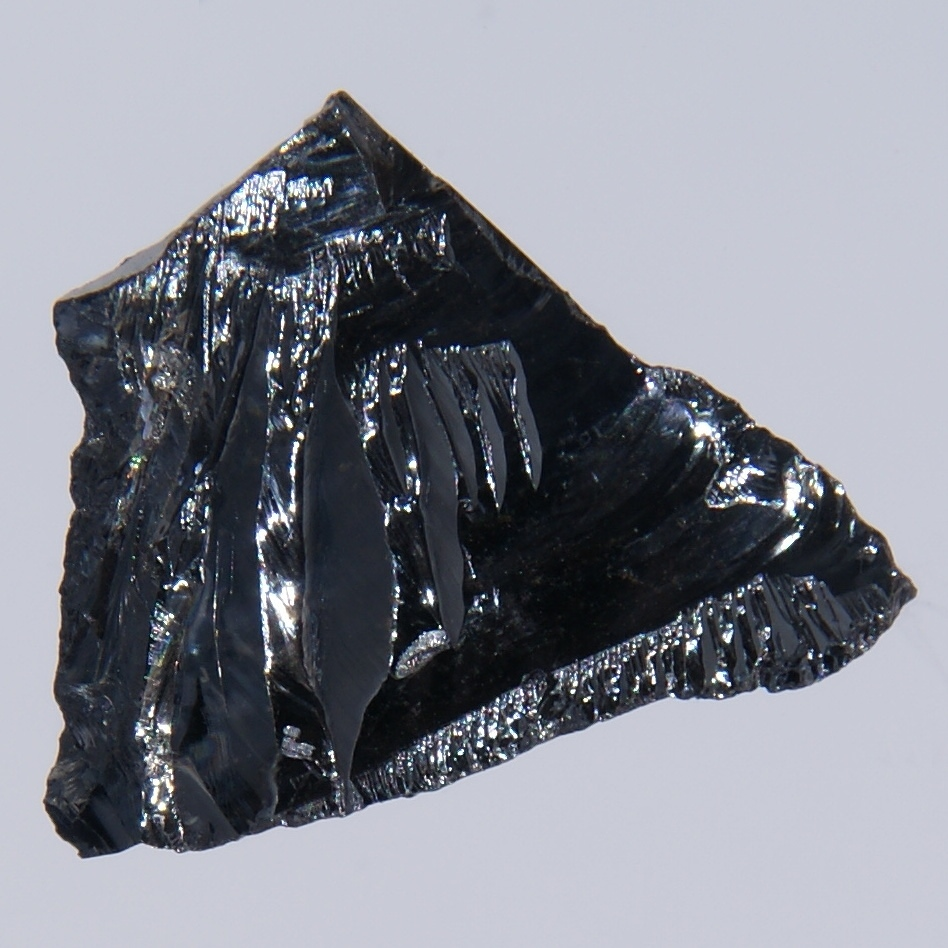
\includegraphics[width=.9\linewidth]{./paso1.jpg}
\end{center}
\end{frame}

\begin{frame}[label={sec:orgf546210}]{Presentacion2}
Paso 2:
Se corta en los extremos para obtener un cilindro perfecto.
Luego se cortan en oleas, del cual se fabrican cientos de procesadores.
\begin{center}
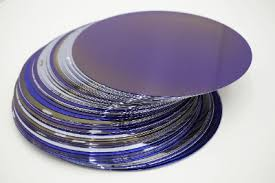
\includegraphics[width=.9\linewidth]{./paso2.jpeg}
\end{center}
\end{frame}

\begin{frame}[label={sec:org04d1dfa}]{Presentacion3}
Paso 3:
Se pulen las oleas para remover defectos/impurezas.
\begin{center}
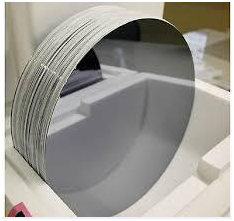
\includegraphics[width=.9\linewidth]{./paso3.png}
\end{center}
\end{frame}

\begin{frame}[label={sec:orga676fec}]{Presentacion4}
Paso 4:
Se dibujan los transistores dentro del wafer que componen el procesador.
\begin{center}
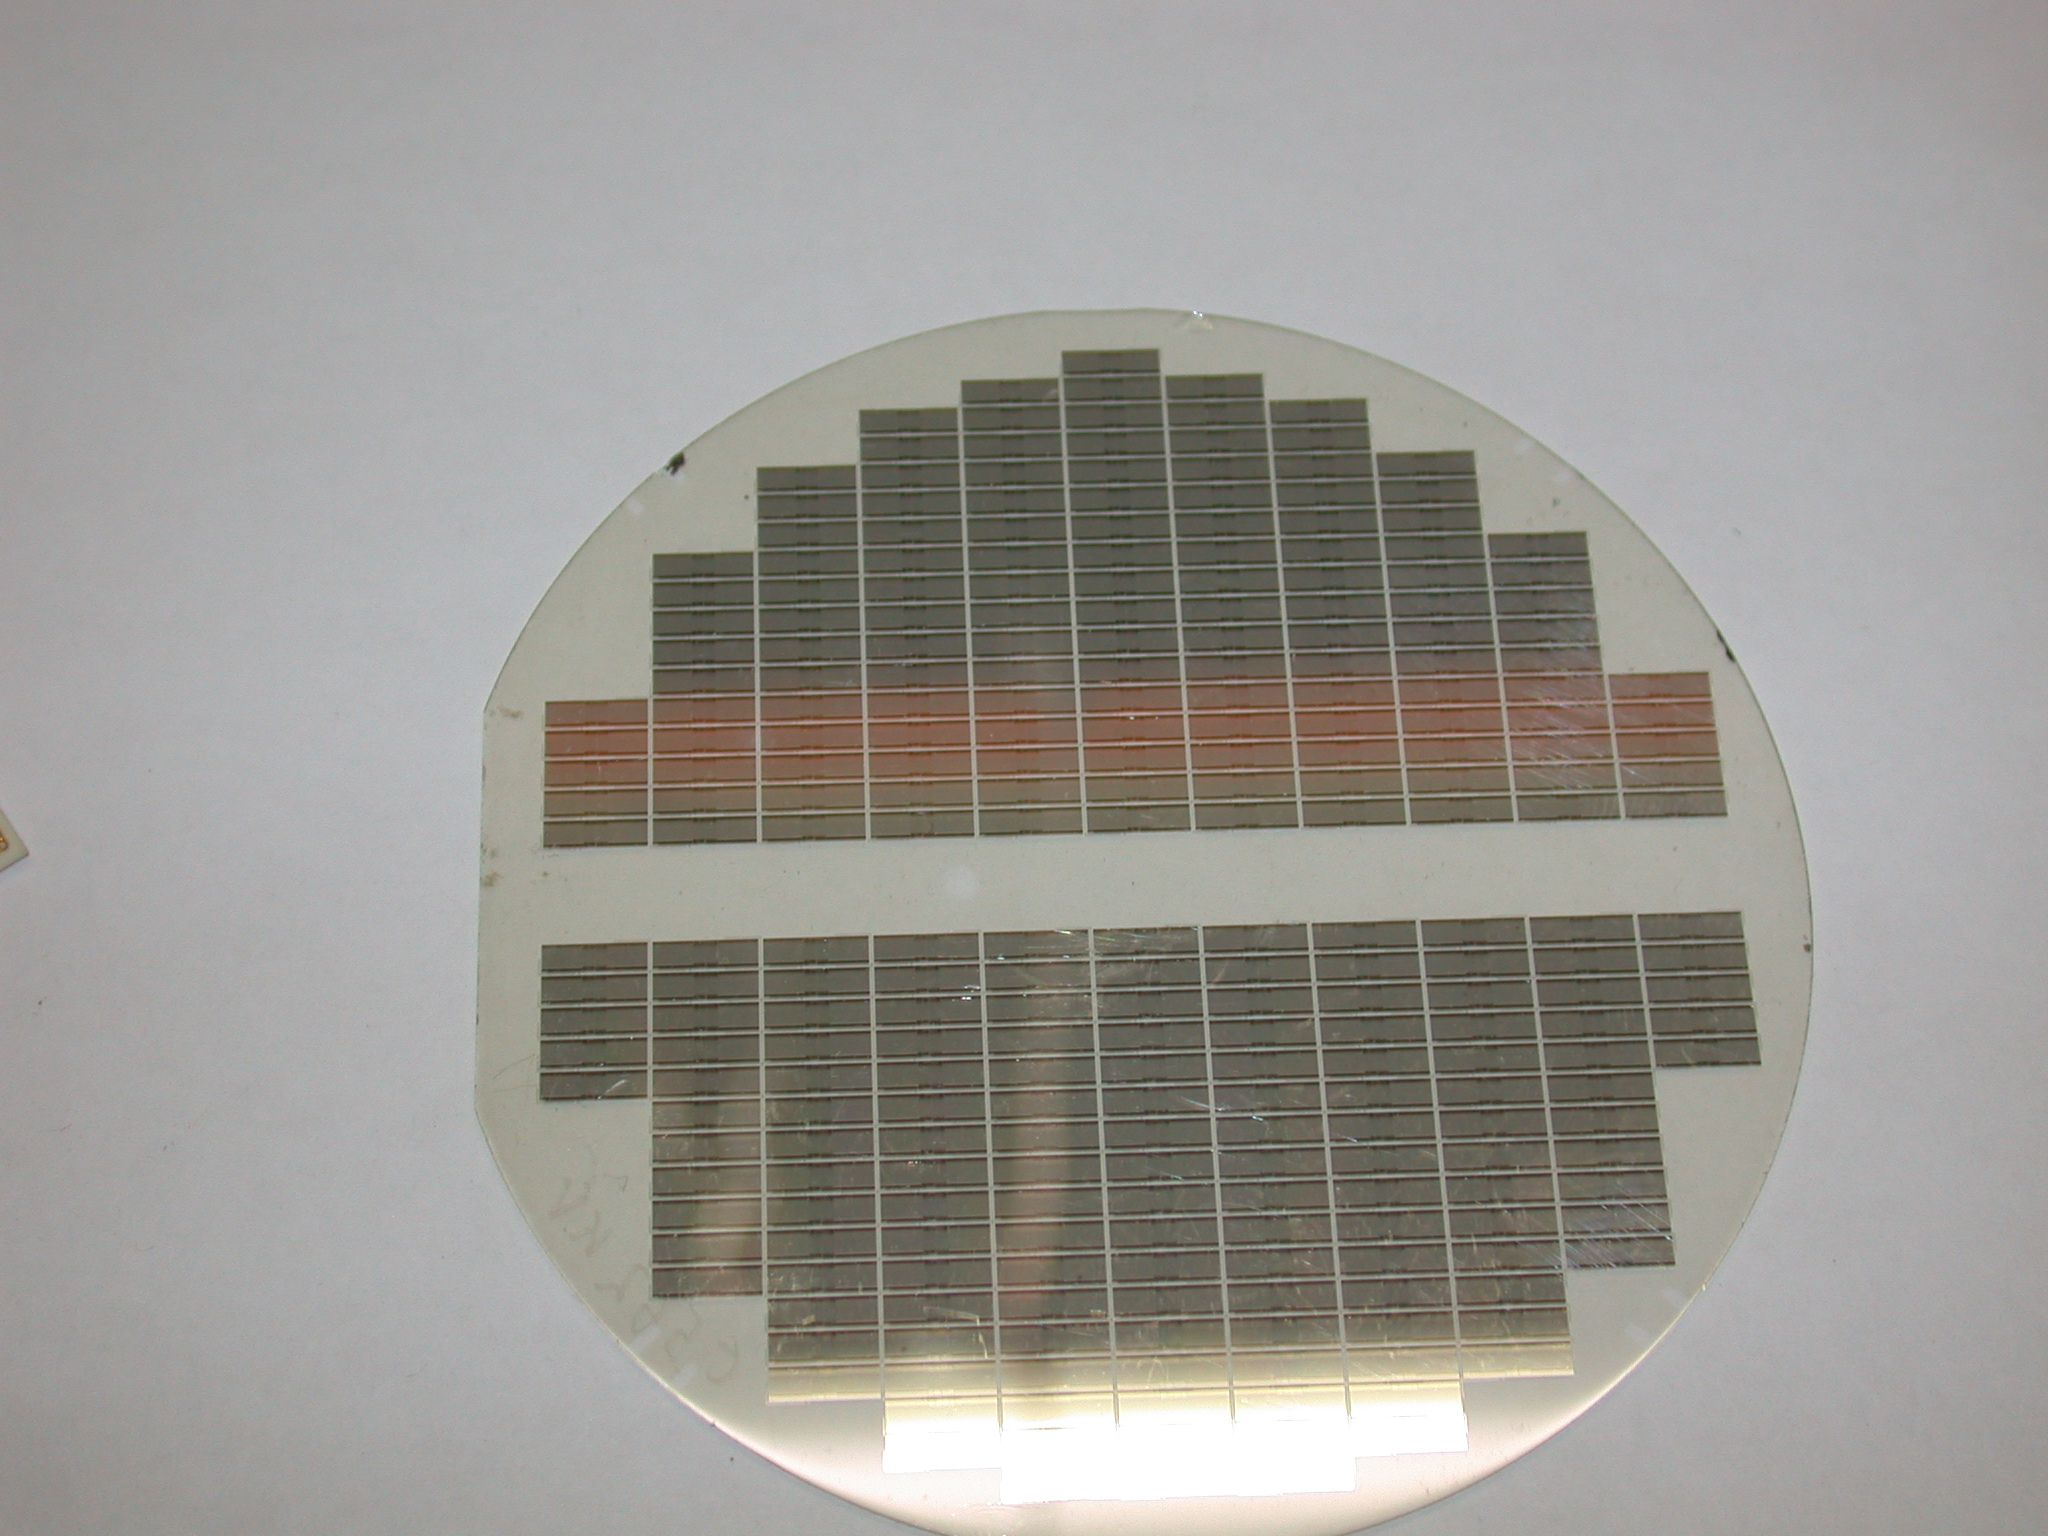
\includegraphics[width=.9\linewidth]{./paso4.jpeg}
\end{center}
\end{frame}

\begin{frame}[label={sec:org2db05cf}]{Presentacion5}
Paso 5:
Se pintan capas sobre el wafer para que reciba el aporte de átomos.
\begin{center}
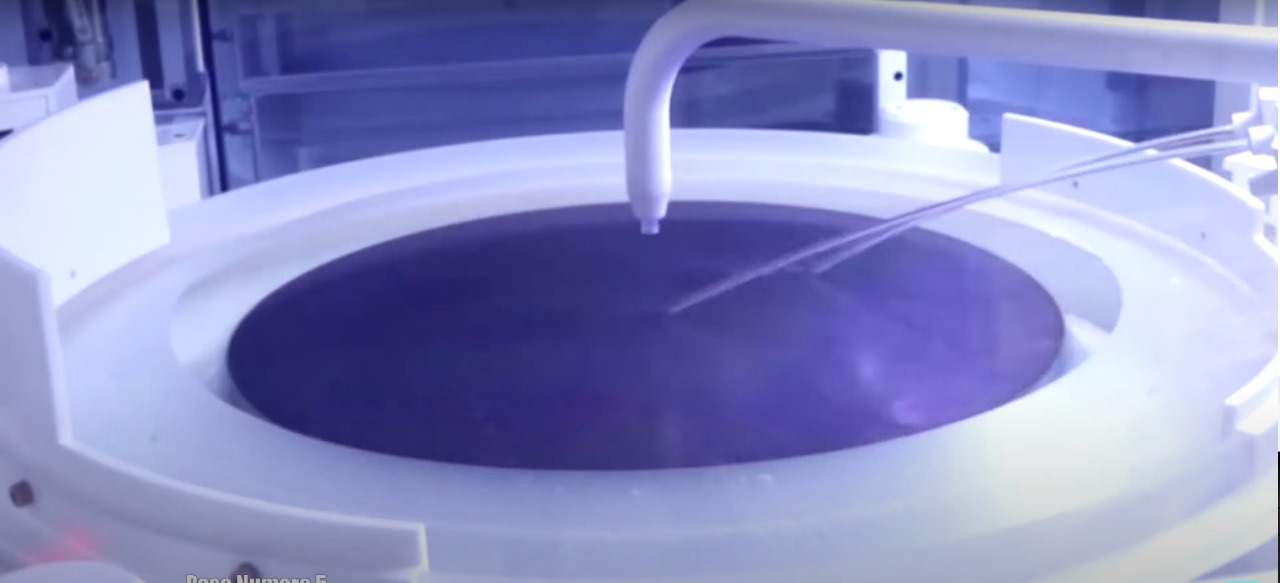
\includegraphics[width=.9\linewidth]{./paso5.jpeg}
\end{center}
\end{frame}

\begin{frame}[label={sec:org25d3c5d}]{Presentacion6}
Paso 6:
Se utiliza luz no visible para el proceso, debido a que la luz es demasiado "grande"
\begin{center}
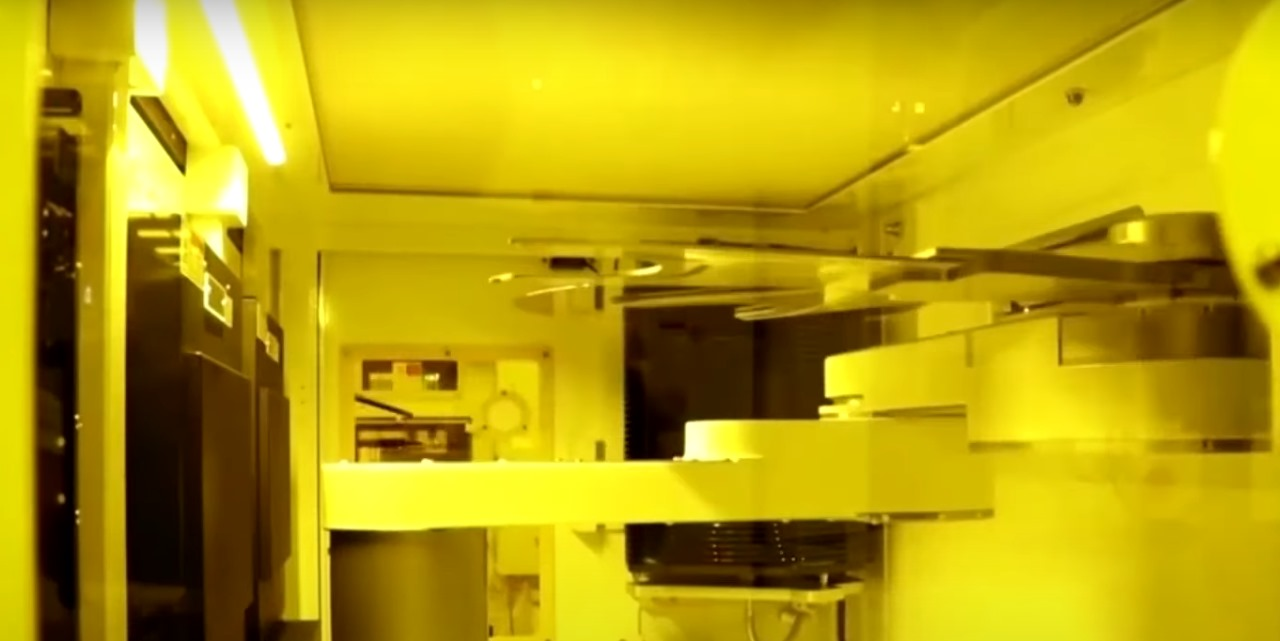
\includegraphics[width=.9\linewidth]{./paso6.jpeg}
\end{center}
\end{frame}

\begin{frame}[label={sec:org88a6a27}]{Presentacion7}
Paso 7:
Despues del proceso litografico que pasó el wafer, se cortan los wafers.
Los microprocesadores extraidos del wafer cortado se individualizan
\begin{center}
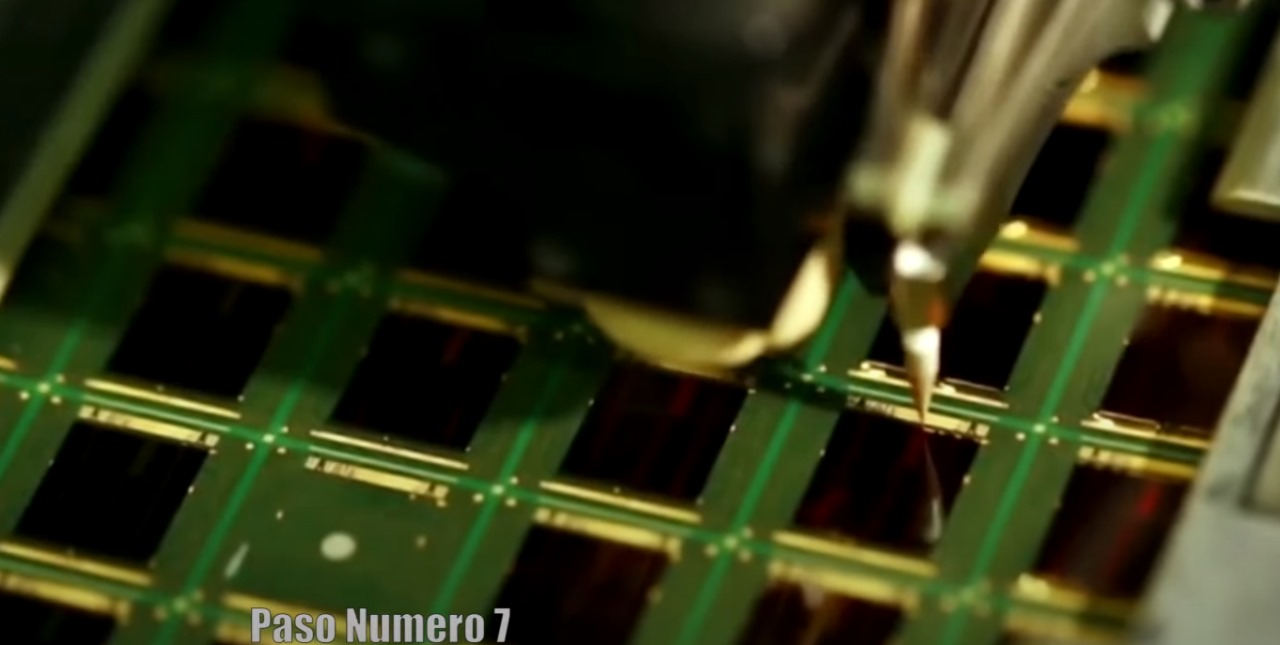
\includegraphics[width=.9\linewidth]{./paso7.jpeg}
\end{center}
\end{frame}

\begin{frame}[label={sec:orga5d1a0e}]{Presentacion8}
Paso 8:
Todo el proceso se realiza en clean rooms.
\begin{center}
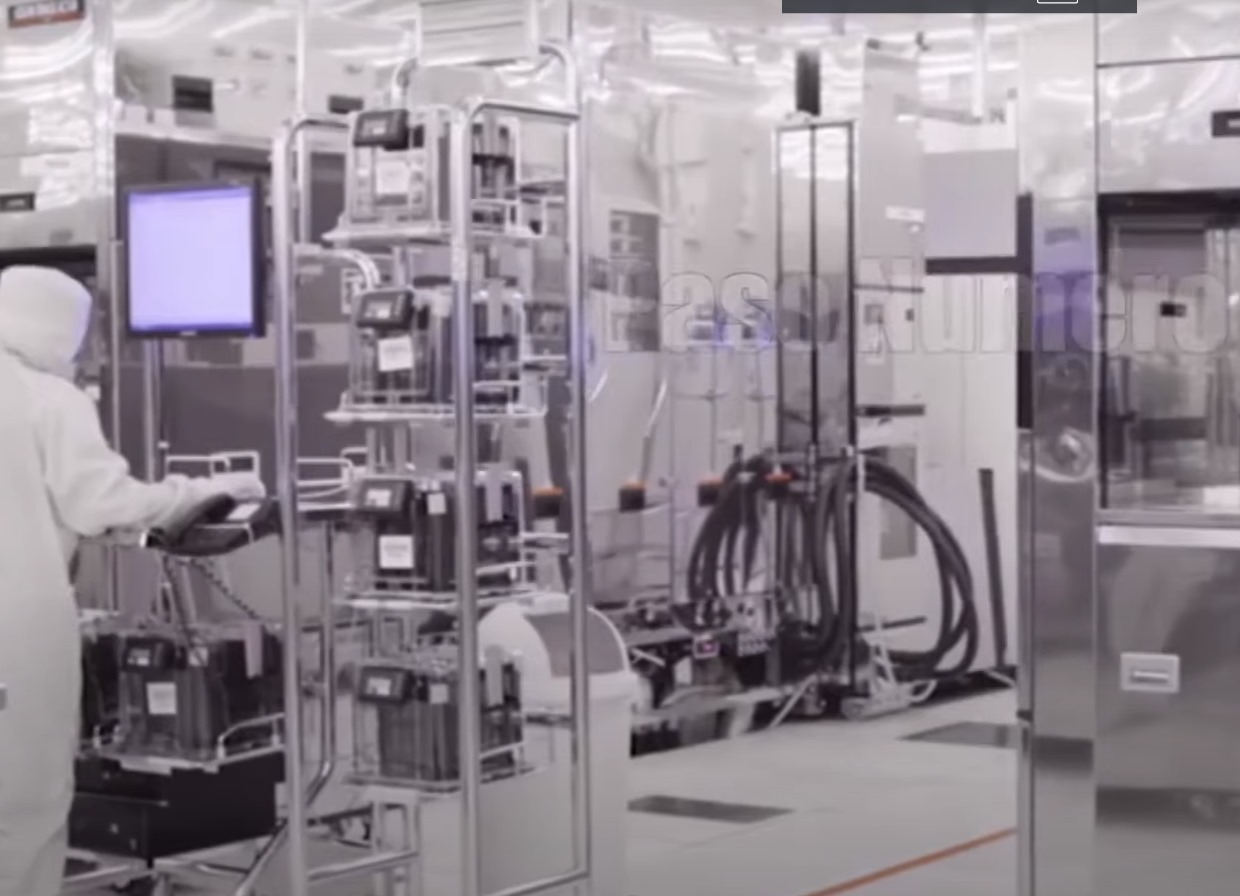
\includegraphics[width=.9\linewidth]{./paso8.jpeg}
\end{center}
\end{frame}

\begin{frame}[label={sec:orgb462fc8}]{Presentacion9}
Paso 9:
Cada placa de los microprocesadores tendra una capsula protectora plastica o ceramica.
Si es necesario la capsula recibira un disipador termico de metal.
\begin{center}
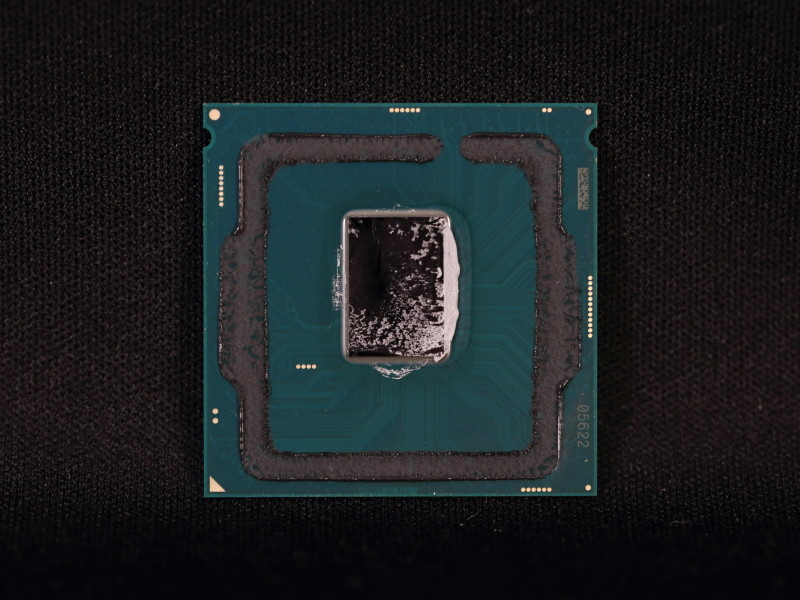
\includegraphics[width=.9\linewidth]{./paso9.jpg}
\end{center}
\end{frame}

\begin{frame}[label={sec:org7e9cda1}]{Paso final}
Paso final:
EL proceso de escrito toma de 2 a 3 meses para ser completados.
De cada cristal de silicio extra puro se obtienen decenas de miles de microprocesadores.
\begin{center}
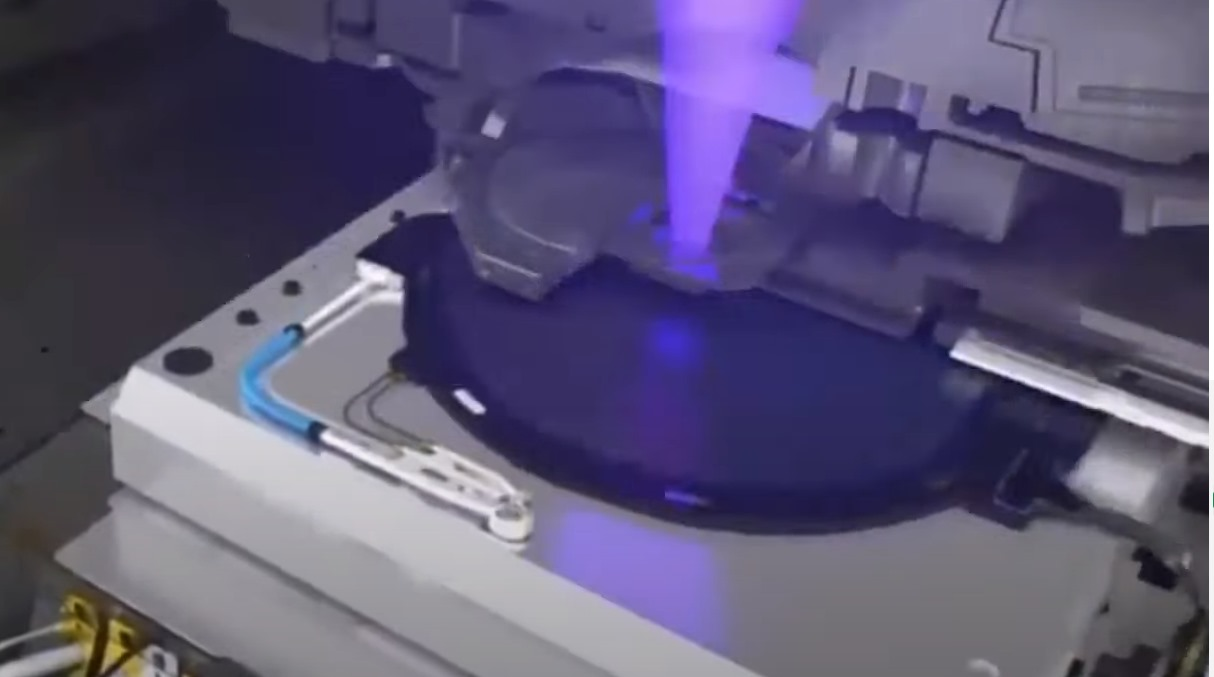
\includegraphics[width=.9\linewidth]{./paso10.jpeg}
\end{center}
\end{frame}
\end{document}
